\begin{figure}[!ht]
    \centering
    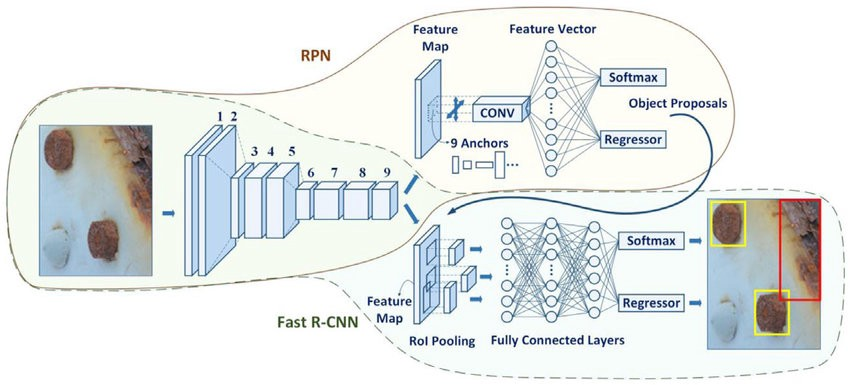
\includegraphics[width=0.9\textwidth]{chapter2/images/faster_rcnn.png}
    \caption{โครงสร้างทั่วไปของโมเดลปัญญาประดิษฐ์ของ Faster RCNN}
    \label{fig:faster_rcnn_architecture}
\end{figure}
\par faster-rcnn มีการพัฒนาในการหาพื้นที่ที่สนใจ (ROI) โดยการเปลี่ยนจากใช้โครงข่ายหาพื้นที่ที่สนใจแยกเฉพาะ (selective search) นำมารวมในโครงข่ายเดียวกัน ดังนั้น faster-rcnn จึงมีโครงข่ายประสาทเทียมเดียวในการทำงาน ซึ่งภายในโครงข่ายจะประกอบไปด้วยการทำงานหลัก 3 อย่าง คือ
\begin{enumerate}
	\setlength\itemsep{-0.25em}
	\item การสกัดคุณลักษณะ
	\\	นำรูปภาพทั้งรูปภาพเข้าโครงข่ายคอนโวลูชั่นเพื่อการสกัดคุณลักษณะของรูปภาพ
	\item การเสนอพื้นที่ที่คาดว่าจะมีวัตถุอยู่
	\\	หลังจากที่รูปภาพผ่านการสกัดคุณลักษณะแล้ว จะถูกนำเข้าไปใน region proposal network เพื่อสร้างข้อเสนอพื้นที่ที่คาดว่าจะมีวัตถุอยู่
	\item การทำนายผล
	\\	ทำการ pooling คุณลักษณะของรูปภาพและพื้นที่ที่คาดว่าจะมีวัตถุอยู่ และ นำเข้าไปในชั้นการทำนายผล (full connected layer) สุดท้ายจะได้ผลลัพธ์เป็นหมวดหมู่ของกรอบสี่เหลี่ยม และ ตำแหน่งของกรอบสี่เหลี่ยม  
\end{enumerate}
\par region proposal network (RPN) คือ โครงข่ายที่เสนอพื้นที่ที่คาดว่าจะมีวัตถุอยู่ จะถูกใช้หลังรูปภาพผ่านการสกัดคุณลักษณะ RPN มีโครงสร้างที่เป็นเอกลักษณ์เฉพาะตัว
คือมีการบอกว่าบริเวณนั้นมีวัตถุอยู่หรือไม่ (classification layer) และ สำหรับการระบุพิกัดของกรอบสี่เหลี่ยมที่คาดว่าจะมีวัตถุอยู่ (regression layer) ซึ่งผลลัพธ์จะได้ ROI (พื้นที่บริเวณที่เราสนใจ)